\begin{frame}{Claimed Versus Effective Context Length}
  \begin{columns}[T,onlytextwidth]
    \column{0.46\textwidth}
      \begin{itemize}\footnotesize\itemsep0.4em
        \item[\textcolor{red}{$\blacktriangleright$}] A model's \textbf{claimed} context length is the longest input it accepts, $n$ tokens. It states a capacity; how much of it the model uses has to be measured.
        \item[\textcolor{red}{$\blacktriangleright$}] RULER, a benchmark of 13 synthetic tasks, defines the \textbf{effective} context length as the longest tested length whose score still clears a pass mark:
          \[ n_{\text{eff}} = \max\{\, n \in \mathcal{N} : a(n) > \tau \,\}, \]
          where $a(n)$ is the mean accuracy over the tasks at length $n$, $\mathcal{N}$ the set of tested lengths (4K to 128K) and $\tau$ the pass mark.
        \item[\textcolor{red}{$\blacktriangleright$}] RULER sets $\tau = 85.6\%$, the score of Llama-2-7B, a 4K-context model, at 4K. In its words, ``almost all models fall below the threshold before reaching the claimed context lengths.''
        \item[\textcolor{red}{$\blacktriangleright$}] $n_{\text{eff}}$ belongs to a benchmark and a threshold; quote both with the number.
      \end{itemize}
    \column{0.52\textwidth}
      \centering
      \vspace{0.6em}
      {\scriptsize
      \setlength{\tabcolsep}{3.5pt}\begin{tabular}{lrrrr}
        \toprule
        \textbf{Model} & \textbf{Claimed} & \textbf{Effective} & \textbf{4K} & \textbf{128K} \\
        \midrule
        Gemini-1.5-Pro & 1M & $>$128K & 96.7 & 94.4 \\
        GPT-4 & 128K & 64K & 96.6 & 81.2 \\
        Llama3.1 (70B) & 128K & 64K & 96.5 & 66.6 \\
        Llama3.1 (8B) & 128K & 32K & 95.5 & 77.0 \\
        Yi (34B) & 200K & 32K & 93.3 & 77.3 \\
        GradientAI/Llama3 (70B) & 1M & 16K & 95.1 & 72.1 \\
        LWM (7B) & 1M & $<$4K & 82.3 & 65.0 \\
        \bottomrule
      \end{tabular}\par}
      \vspace{0.5em}
      {\scriptsize Mean accuracy (\%) over the 13 tasks at 4K and 128K tokens. LWM (7B) starts below the pass mark at 4K, so its effective length is under 4K although it degrades slowly.\par}
      \vspace{0.6em}
      {\scriptsize Hsieh et al., ``RULER: What's the Real Context Size of Your Long-Context Language Models?'' COLM 2024, \href{https://arxiv.org/abs/2404.06654v3}{arXiv:2404.06654v3}, Sections~1 and~4, Table~3.\par}
  \end{columns}
\end{frame}

\begin{frame}{Lost in the Middle}
  \begin{columns}[T,onlytextwidth]
    \column{0.52\textwidth}
      \begin{itemize}\footnotesize\itemsep0.35em
        \item[\textcolor{red}{$\blacktriangleright$}] Liu et al. measured the edge bias under controlled conditions. Each prompt holds $p$ Wikipedia passages of at most 100 tokens: one answers a NaturalQuestions-Open question, and the other $p-1$ are the passages a retriever ranks highest among those without the answer. Only the position of the answering passage changes.
        \item[\textcolor{red}{$\blacktriangleright$}] GPT-3.5-Turbo with $p = 20$ is right 75.8\% of the time with the passage first, 63.2\% with it last, and 53.8\% at position 10: a U-shaped curve of primacy and recency.
        \item[\textcolor{red}{$\blacktriangleright$}] With no passages (closed book) it scores 56.1\%; with only the answering passage, 88.3\%. At position 10 it does worse than with no passages at all.
        \item[\textcolor{red}{$\blacktriangleright$}] A longer window does not change the curve. GPT-3.5-Turbo (16K) and Claude-1.3 (100K) score almost exactly like their 4K and 8K versions on inputs that fit in both.
        \item[\textcolor{red}{$\blacktriangleright$}] What to report: accuracy as a function of position, and the gap between the best and the worst position. An average over positions hides the middle.
      \end{itemize}
    \column{0.46\textwidth}
      \centering
      \vspace{0.2em}
      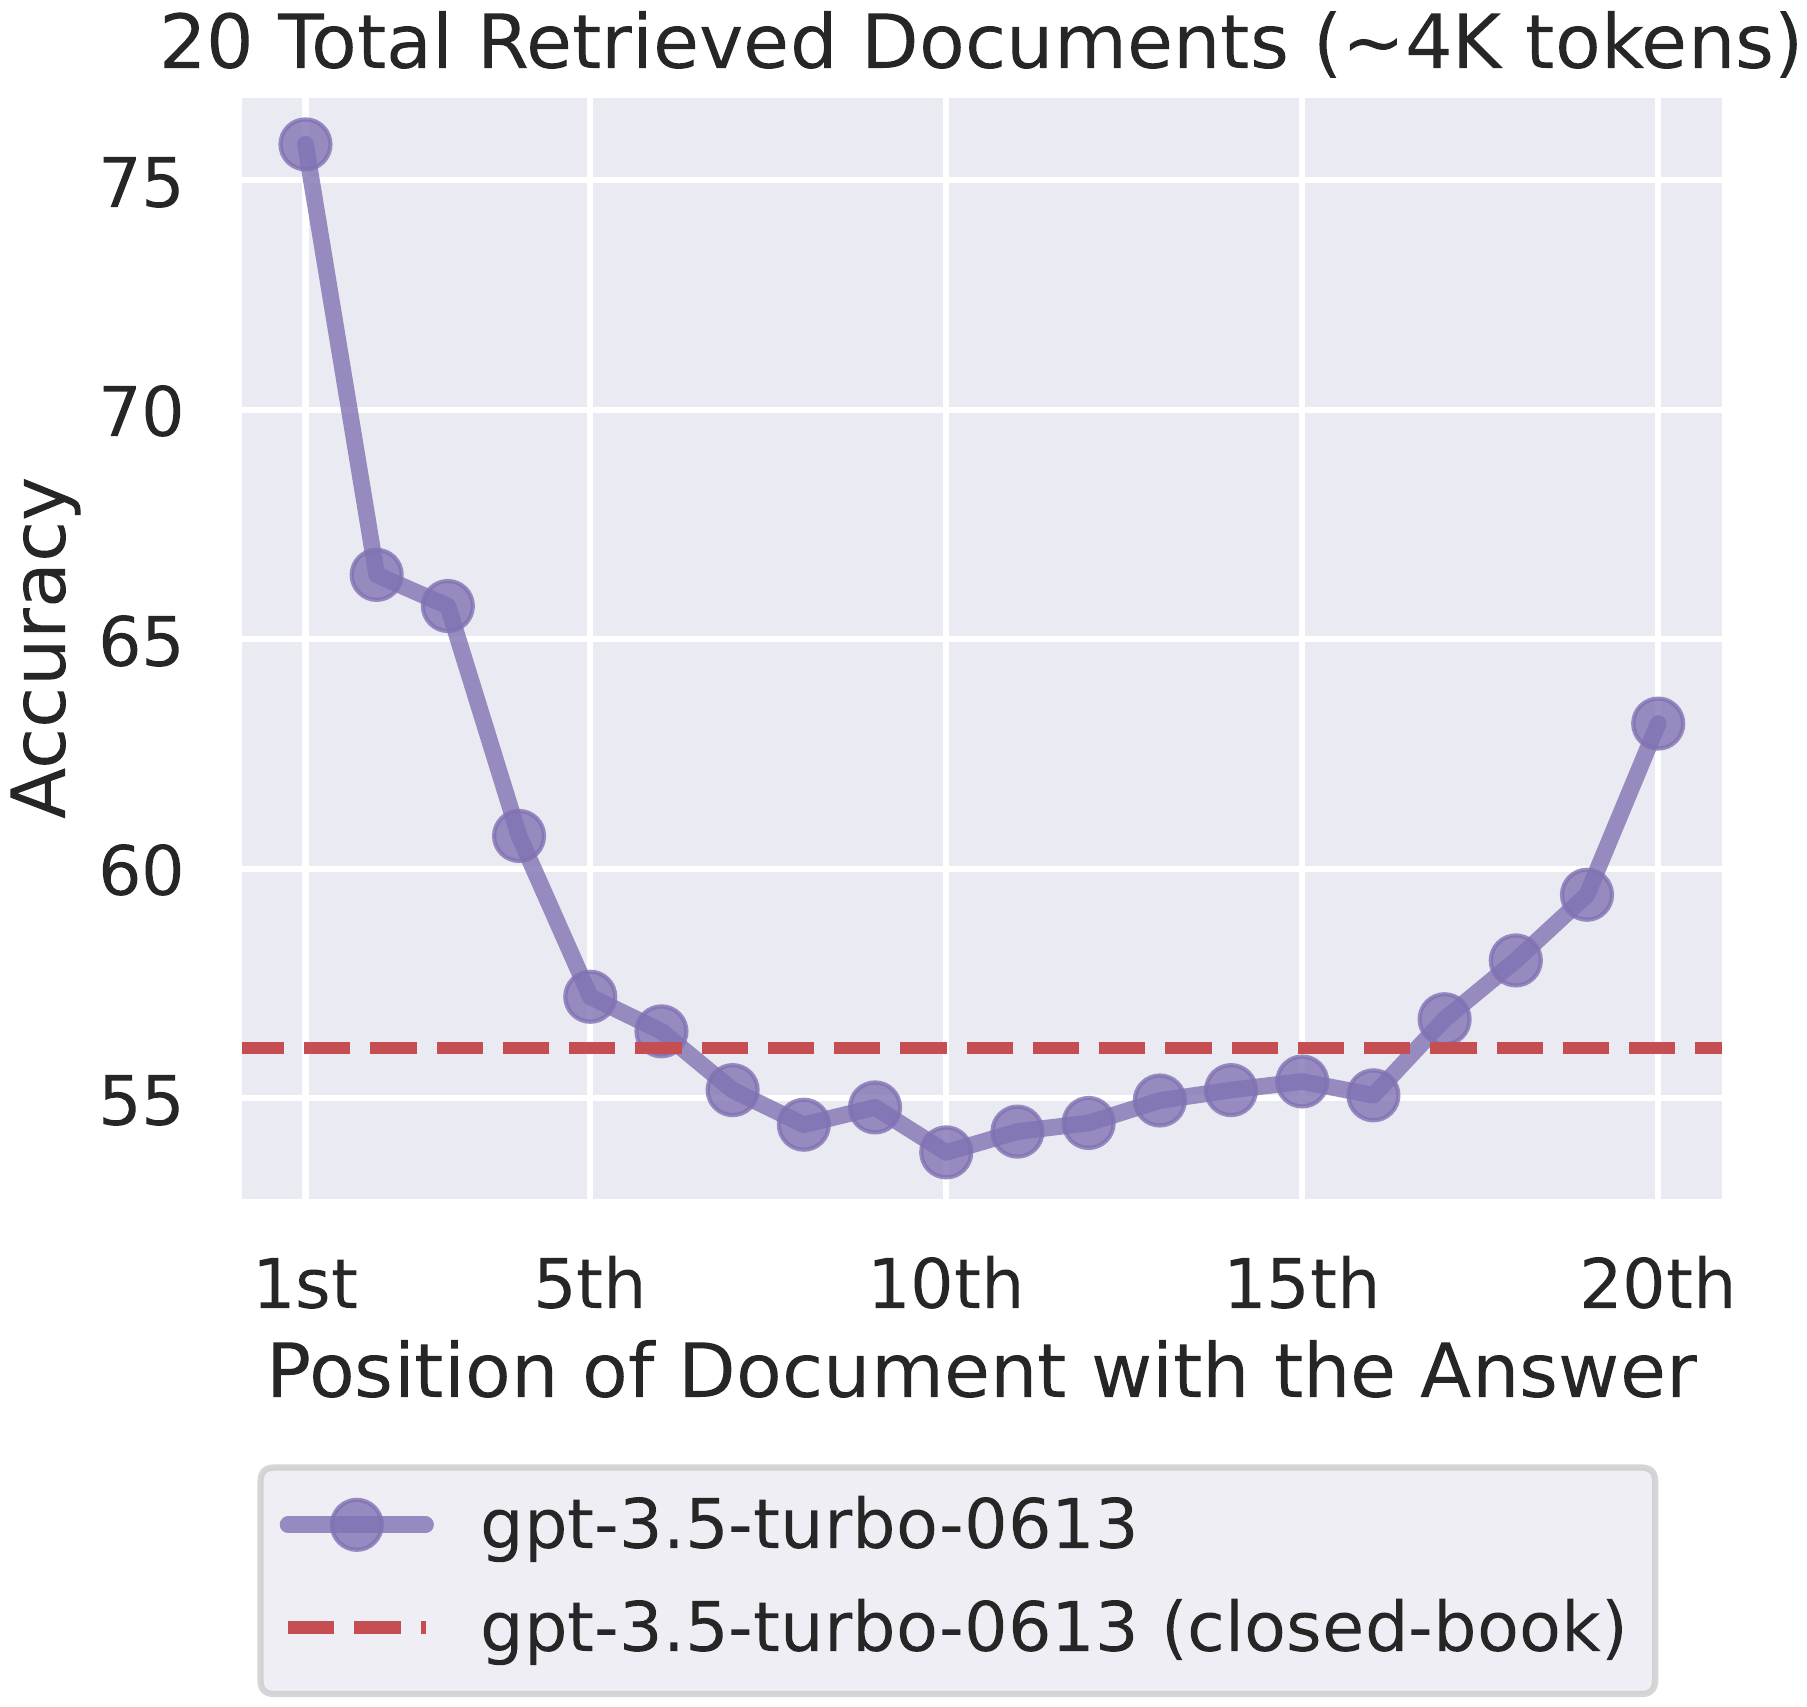
\includegraphics[width=\linewidth,height=0.62\textheight,keepaspectratio]{images/long-context/litm_fig1_position_u_curve.png}\\[0.2em]
      {\scriptsize Accuracy against the position of the answering passage; the dashed line is closed-book accuracy. Liu et al., ``Lost in the Middle: How Language Models Use Long Contexts,'' TACL 2024, \href{https://arxiv.org/abs/2307.03172v3}{arXiv:2307.03172v3}, Figure~1; numbers from Tables~1 and~6.\par}
  \end{columns}
\end{frame}

\begin{frame}{The Needle-in-a-Haystack Test}
  \begin{columns}[T,onlytextwidth]
    \column{0.44\textwidth}
      \begin{itemize}\scriptsize\itemsep0.3em
        \item[\textcolor{red}{$\blacktriangleright$}] \textbf{Needle in a haystack (NIAH)}, released by Greg Kamradt in November 2023: insert one sentence, the needle, at depth $x\%$ of a haystack of Paul Graham essays cut to $n$ tokens, ask for it, and sweep $x$ and $n$ into a heatmap.
        \item[\textcolor{red}{$\blacktriangleright$}] Needle: ``The best thing to do in San Francisco is eat a sandwich and sit in Dolores Park on a sunny day.'' Question: ``What is the best thing to do in San Francisco?'' (``most fun thing'' in the code released in November 2023). An LLM judge scores the answer from 1 to 10.
        \item[\textcolor{red}{$\blacktriangleright$}] It tests literal retrieval of one fact. On GPT-4 128K, accuracy ``started to degrade at large context lengths when the fact was placed between 10\%--50\% document depth''.
        \item[\textcolor{red}{$\blacktriangleright$}] A pass is weak evidence: the question repeats the needle's words, there is one fact and nothing to combine, and recent models score near-perfectly.
        \item[\textcolor{red}{$\blacktriangleright$}] Models with ``nearly perfect accuracy in the vanilla NIAH test'' still show ``large performance drops as the context length increases'' on RULER. Across 59 models, HELMET finds that ``synthetic tasks like NIAH do not reliably predict downstream performance.''
      \end{itemize}
    \column{0.54\textwidth}
      \centering
      \vspace{0.6em}
      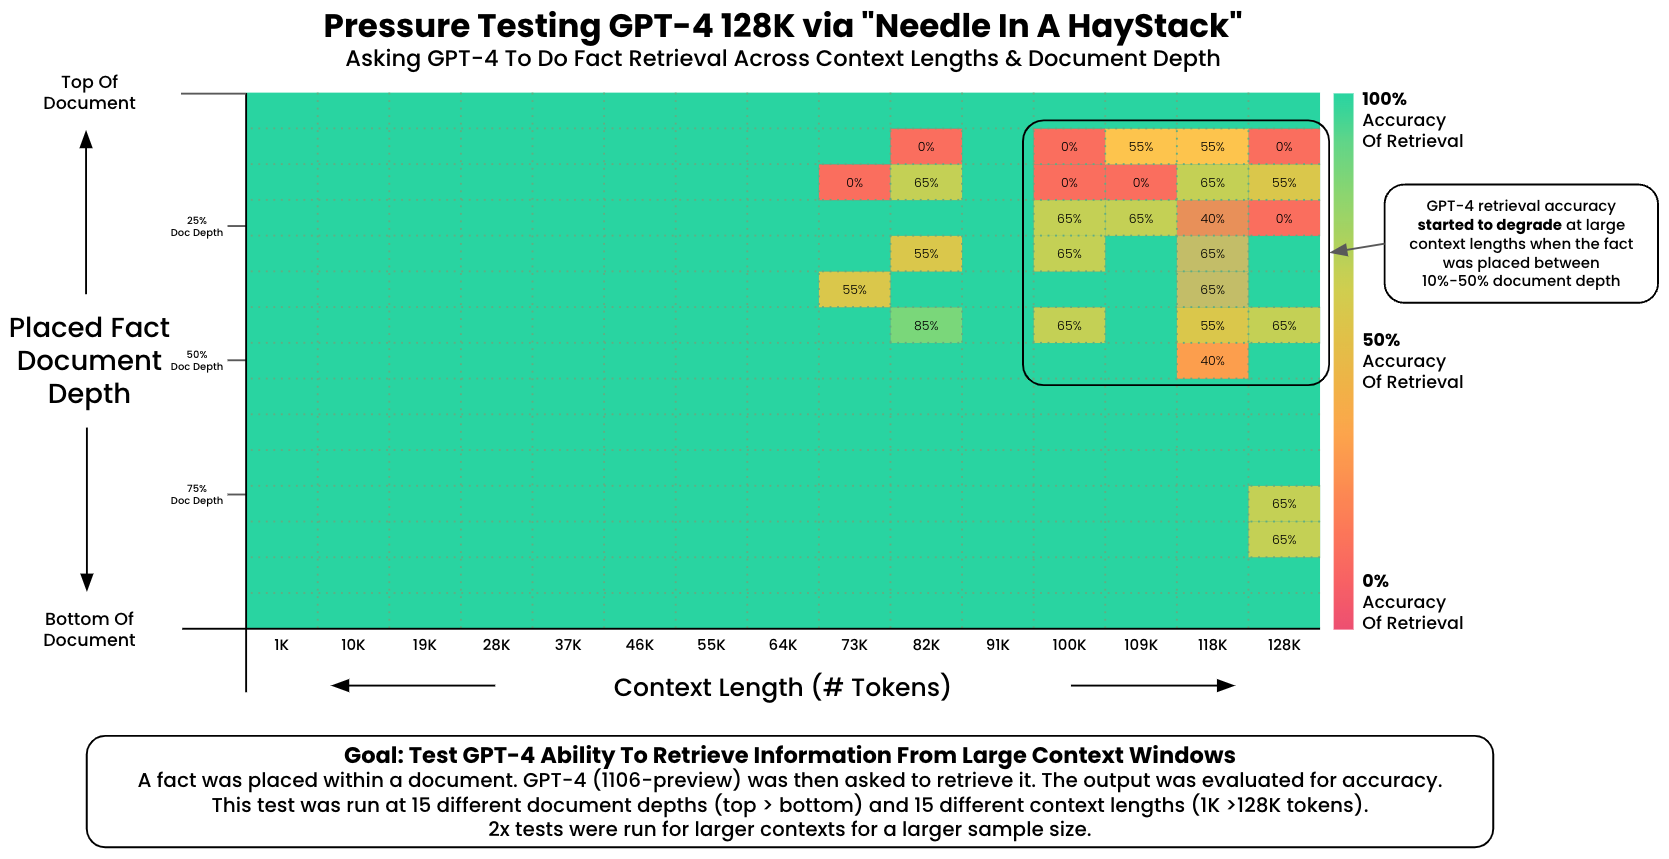
\includegraphics[width=\linewidth,height=0.56\textheight,keepaspectratio]{images/long-context/niah_gpt4_128k_heatmap.png}\\[0.2em]
      {\scriptsize Source: G.~Kamradt, \texttt{needle-in-a-haystack} repository, \href{https://github.com/gkamradt/needle-in-a-haystack}{github.com/gkamradt/needle-in-a-haystack} (\texttt{img/GPT\_4\_testing.png}), run of 8~Nov.\ 2023, MIT licence.\par}
      \vspace{0.6em}
      {\scriptsize Quotes: Hsieh et al., \href{https://arxiv.org/abs/2404.06654v3}{arXiv:2404.06654v3}, abstract; Yen et al., ``HELMET: How to Evaluate Long-Context Language Models Effectively and Thoroughly,'' ICLR 2025, \href{https://arxiv.org/abs/2410.02694v3}{arXiv:2410.02694v3}, abstract.\par}
  \end{columns}
\end{frame}

\begin{frame}{RULER: Thirteen Tasks Beyond One Needle}
  \begin{columns}[T,onlytextwidth]
    \column{0.47\textwidth}
      \begin{itemize}\scriptsize\itemsep0.3em
        \item[\textcolor{red}{$\blacktriangleright$}] Synthetic tasks with controllable length and difficulty: 500 examples per task at each length from 4K to 128K, and an answer counts when it contains the target. Four categories:\par
          \begin{itemize}\scriptsize\itemsep0.1em
            \item \textbf{Retrieval:} NIAH with word, number or UUID (random 32-digit identifier) needles; extra needles with other keys as distractors; several values or several keys to return.
            \item \textbf{Multi-hop tracing:} in ``VAR X1 = 12345 \ldots{} VAR X2 = X1 \ldots{} VAR X3 = X2'', name every variable that holds 12345.
            \item \textbf{Aggregation:} return the most frequent words of a long word list, a proxy for summarization.
            \item \textbf{Question answering:} the paragraphs that answer SQuAD and HotpotQA questions, hidden among other paragraphs of the same dataset.
          \end{itemize}
        \item[\textcolor{red}{$\blacktriangleright$}] The 17 models tested all claim 32K or more, yet ``only half of them can maintain satisfactory performance at the length of 32K'' (10 of the 17 in Table~3).
        \item[\textcolor{red}{$\blacktriangleright$}] Yi-34B claims 200K and keeps 100\% on passkey retrieval (a number hidden in repeated filler text) and vanilla NIAH up to 256K. UUID needles and distractor keys pull it down; with the haystack full of distractor needles it loses 40 points at 256K.
      \end{itemize}
    \column{0.51\textwidth}
      \centering
      \vspace{1.0em}
      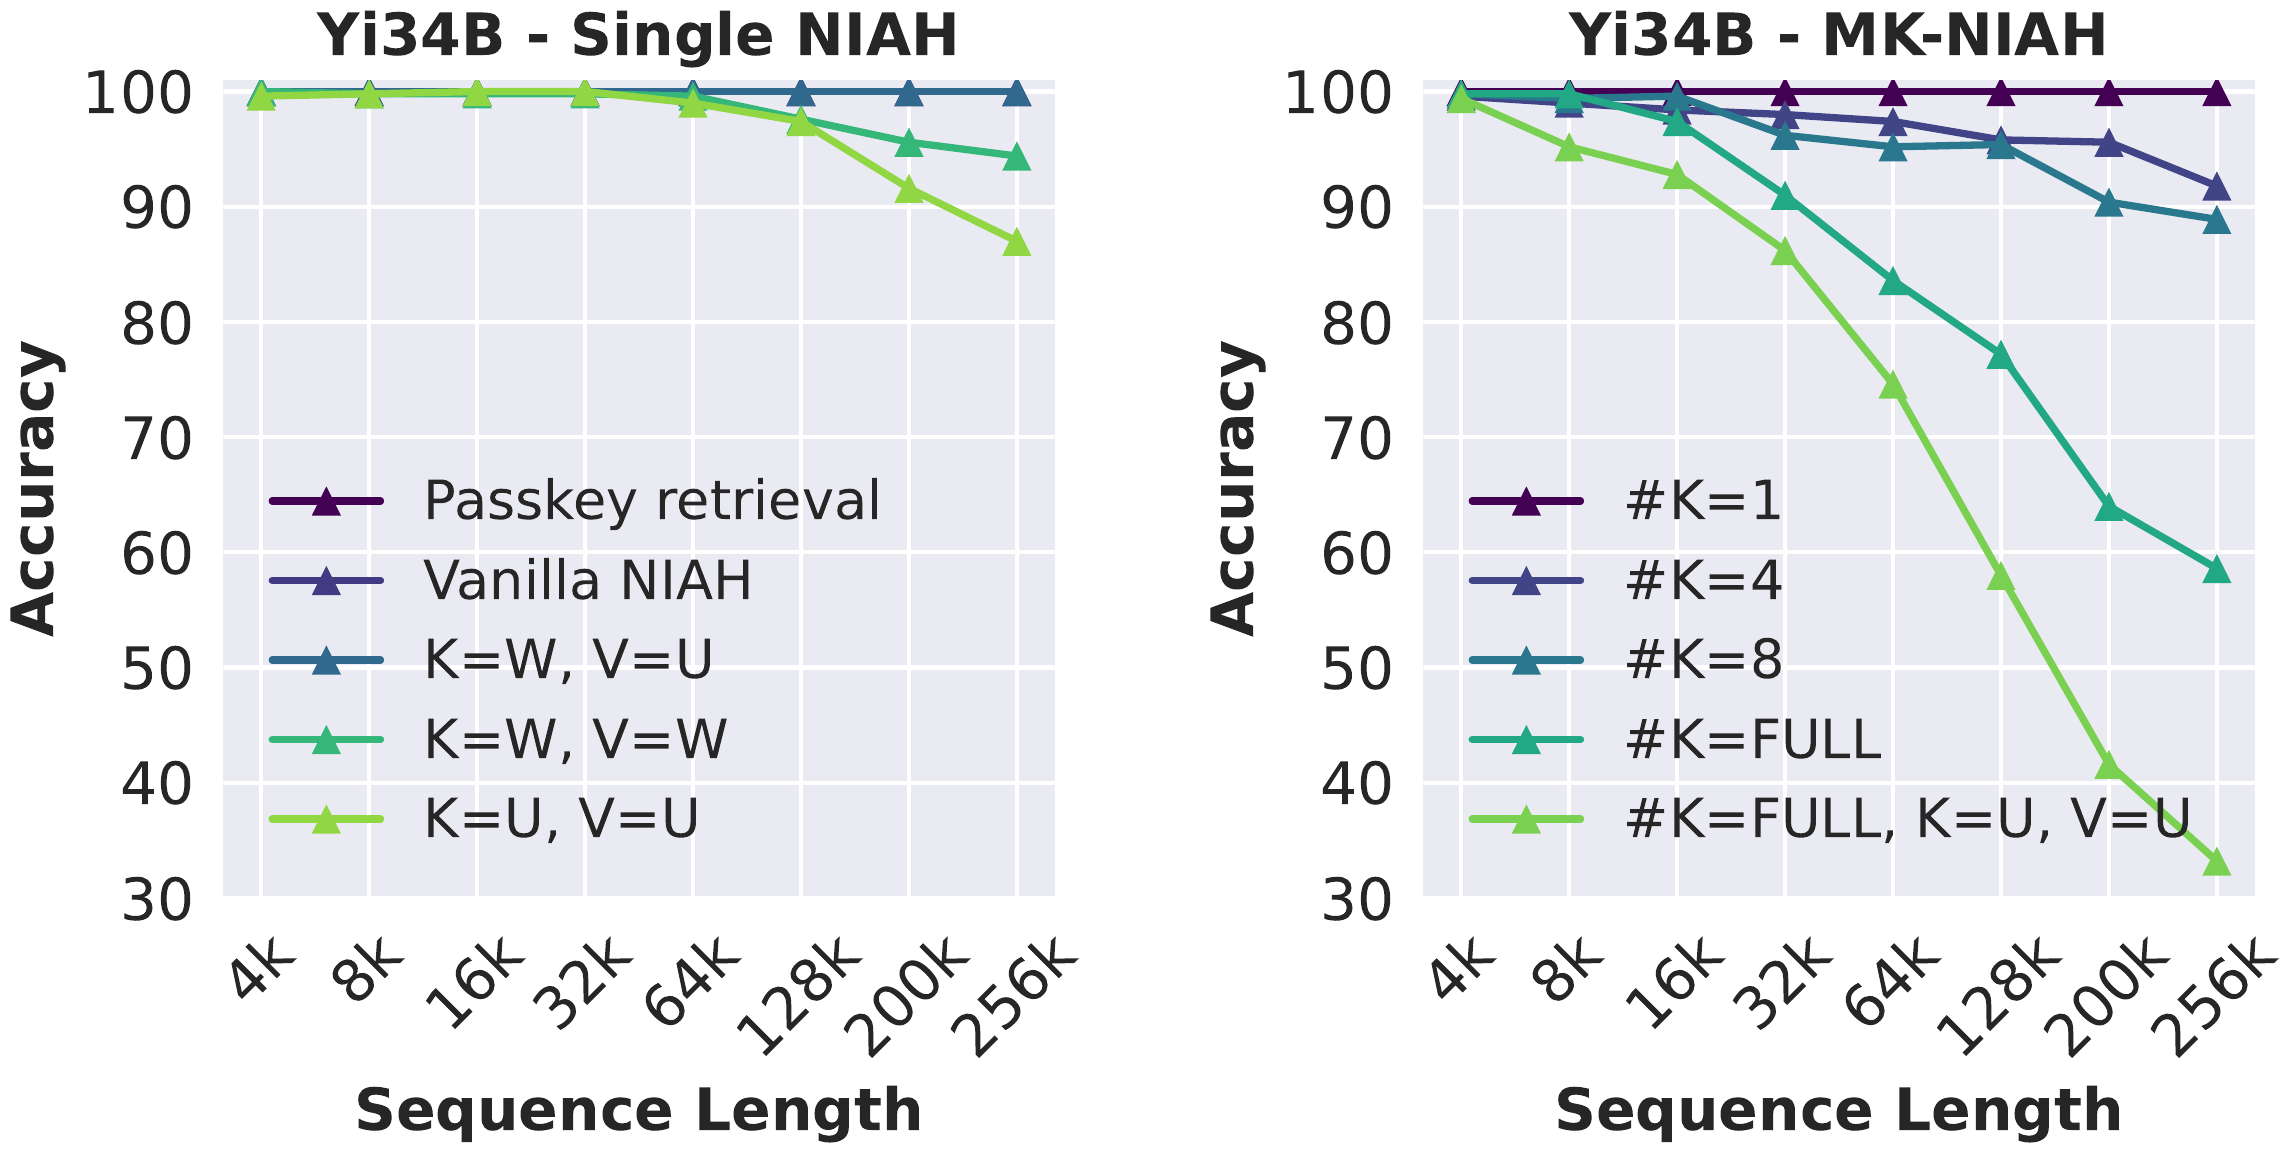
\includegraphics[width=\linewidth,height=0.55\textheight,keepaspectratio]{images/long-context/ruler_fig2ab_yi34b_niah_variants.png}\\[0.2em]
      {\scriptsize Yi-34B with different needle types (left; K and V give the key and value type: W words, U UUIDs) and with $\#K$ keys, one of them the target (right). Hsieh et al., \href{https://arxiv.org/abs/2404.06654v3}{arXiv:2404.06654v3}, Figure~2, first two of four panels.\par}
  \end{columns}
\end{frame}

\begin{frame}{BABILong: Reasoning Over Scattered Facts}
  \begin{columns}[T,onlytextwidth]
    \column{0.58\textwidth}
      \begin{itemize}\scriptsize\itemsep0.3em
        \item[\textcolor{red}{$\blacktriangleright$}] Start from a bAbI task (Weston et al., 2016): a short generated story about people, objects and places, followed by a question. Hide the story's sentences, in order, between sentences of books from the PG19 corpus until the sample is $n$ tokens long.
        \item[\textcolor{red}{$\blacktriangleright$}] 20 tasks: fact chaining, induction, deduction, counting, lists and sets. QA1 needs one supporting fact, QA2 two and QA3 three; the story's other facts act as distractors. Ready-made splits go up to 10M tokens, and the generator extends to any length.
        \item[\textcolor{red}{$\blacktriangleright$}] Order matters. In the figure, F1 and F3 both mention Mary, and only the later one answers ``Where is Mary?''. Because the facts are generated, they cannot have leaked into pre-training data.
        \item[\textcolor{red}{$\blacktriangleright$}] Pass mark: 85\% accuracy. Of 34 LLMs tested without fine-tuning on BABILong, most pass QA1 only up to 4K tokens and the best hold to 64K; with background text none reaches 85\% on QA2, and the best QA3 score stays below 80\%.
        \item[\textcolor{red}{$\blacktriangleright$}] The authors' summary: ``popular LLMs effectively utilize only 10--20\% of the context.'' BABILong is also used to test memory-based models.
      \end{itemize}
    \column{0.40\textwidth}
      \centering
      \vspace{0.2em}
      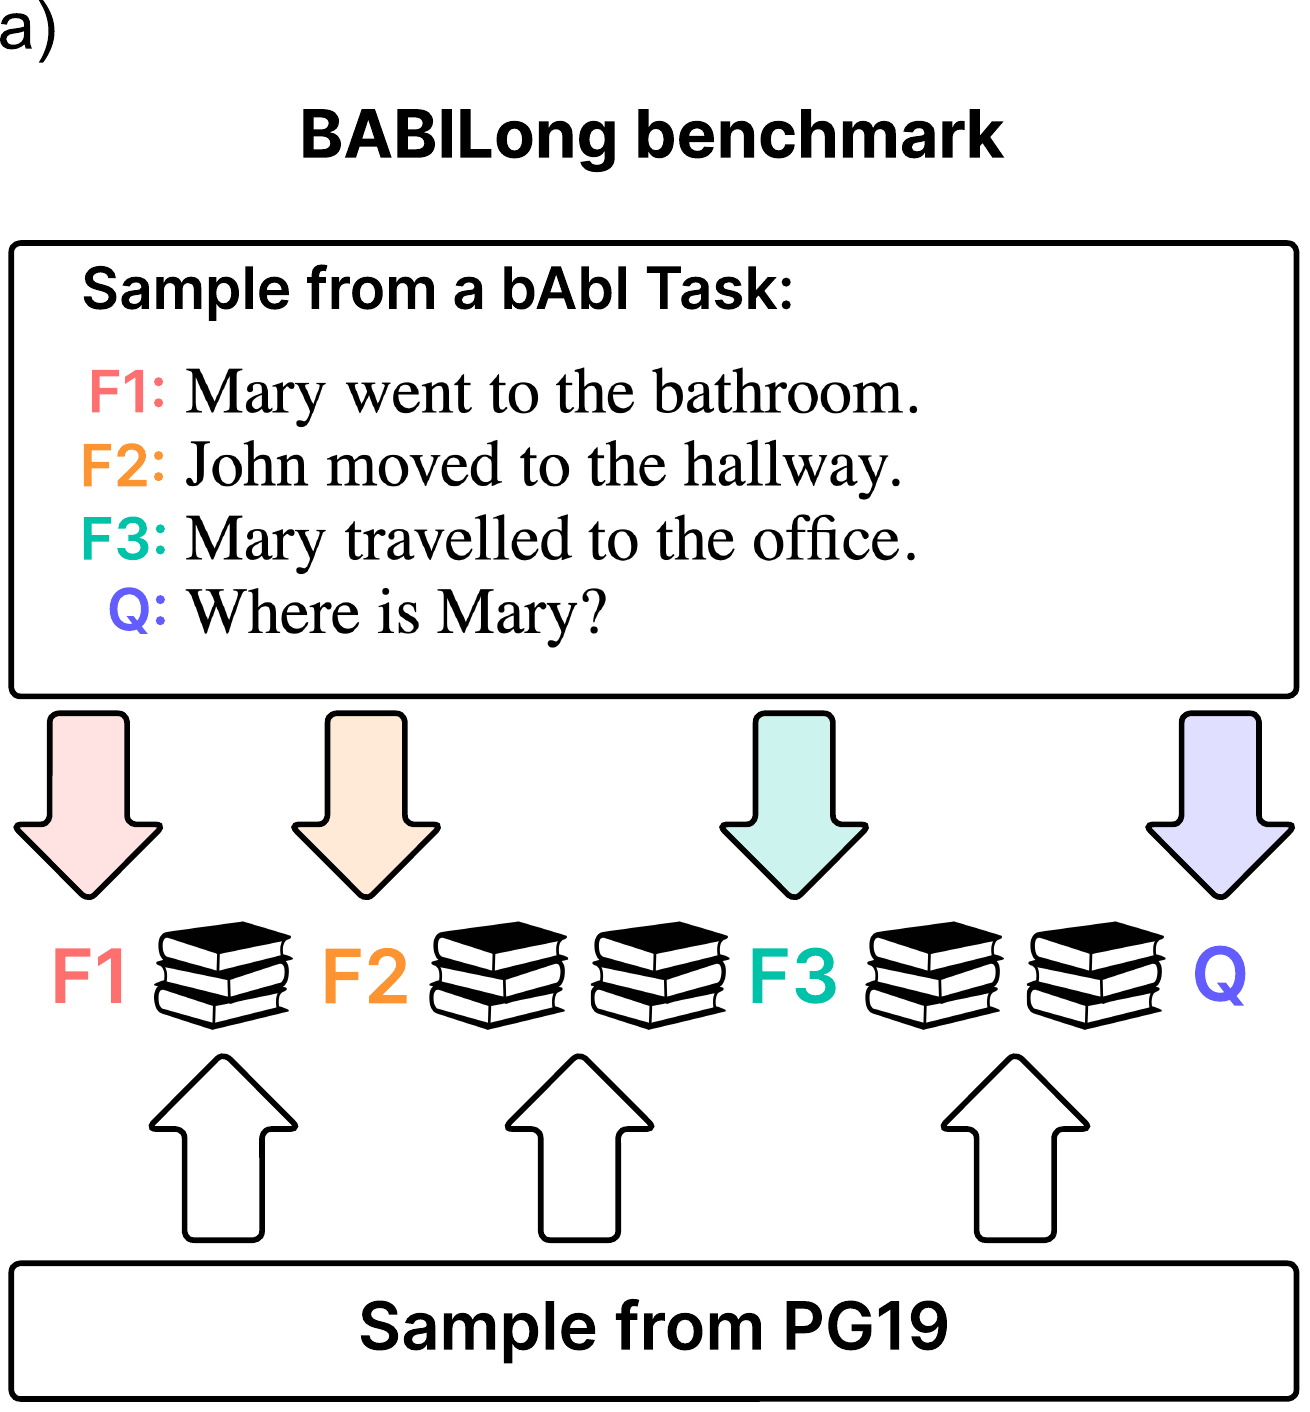
\includegraphics[width=\linewidth,height=0.62\textheight,keepaspectratio]{images/long-context/babilong_fig1a_construction.png}\\[0.2em]
      {\scriptsize Kuratov et al., ``BABILong: Testing the Limits of LLMs with Long Context Reasoning-in-a-Haystack,'' NeurIPS 2024 Datasets and Benchmarks, \href{https://arxiv.org/abs/2406.10149v2}{arXiv:2406.10149v2}, Figure~1(a); numbers from the abstract, Table~1 and Section~3.1.\par}
  \end{columns}
\end{frame}

\begin{frame}{NoLiMa: Needles Without Literal Overlap}
  \begin{columns}[T,onlytextwidth]
    \column{0.52\textwidth}
      \begin{itemize}\scriptsize\itemsep0.3em
        \item[\textcolor{red}{$\blacktriangleright$}] The question shares no keyword with the needle; linking them takes one or two steps of world knowledge or common sense.\par
          \begin{itemize}\scriptsize\itemsep0.05em
            \item Needle: ``Actually, Yuki lives next to the Semper Opera House.''
            \item One hop: ``Which character has been to Dresden?''
            \item Two hops: ``Which character has been to the state of Saxony?''
          \end{itemize}
        \item[\textcolor{red}{$\blacktriangleright$}] Overlap as ROUGE-1 precision, the share of the question's words that also occur in the needle: 0.905 for vanilla NIAH, 0.571 for RULER's single needle, 0.553 for BABILong, 0.069 for NoLiMa.
        \item[\textcolor{red}{$\blacktriangleright$}] Haystacks are snippets of 10 open-license books, filtered so that no other sentence answers the question. 58 question--needle pairs, 26 needle positions, lengths from 250 to 32K tokens.
        \item[\textcolor{red}{$\blacktriangleright$}] The pass mark is relative: 85\% of each model's own score at 250 to 1K tokens. Of 13 models claiming at least 128K, 11 score at most half of their short-context score at 32K. GPT-4o falls from 99.3\% to 69.7\% and is effective only to 8K.
      \end{itemize}
    \column{0.46\textwidth}
      \centering
      \vspace{0.6em}
      {\scriptsize Llama~3.3 70B, accuracy (\%) by context length\\[0.3em]
      \setlength{\tabcolsep}{4pt}\begin{tabular}{lrrr}
        \toprule
        \textbf{Question} & \textbf{8K} & \textbf{16K} & \textbf{32K} \\
        \midrule
        Direct (keyword in question) & 98.3 & 98.5 & 98.5 \\
        One hop & 84.1 & 73.2 & 56.2 \\
        Two hops & 57.4 & 42.7 & 25.9 \\
        \bottomrule
      \end{tabular}\par}
      \vspace{0.6em}
      \begin{itemize}\scriptsize\itemsep0.3em
        \item[\textcolor{red}{$\blacktriangleright$}] Same needles and haystacks; only the question changes. With the needle's keyword in the question, accuracy stays flat to 32K.
        \item[\textcolor{red}{$\blacktriangleright$}] For two-hop questions, accuracy falls with context length even when the needle stays in the last 2K tokens, at a fixed distance from the question, so position alone does not explain the drop.
      \end{itemize}
      \vspace{0.3em}
      {\scriptsize Modarressi et al., ``NoLiMa: Long-Context Evaluation Beyond Literal Matching,'' ICML 2025, \href{https://arxiv.org/abs/2502.05167v3}{arXiv:2502.05167v3}, Sections~3 and~4, Tables~1, 3 and~6.\par}
  \end{columns}
\end{frame}

\begin{frame}{Extending the Window Is the Cheap Part}
  \begin{columns}[T,onlytextwidth]
    \column{0.52\textwidth}
      \begin{itemize}\scriptsize\itemsep0.35em
        \item[\textcolor{red}{$\blacktriangleright$}] Fu et al. take LLaMA-2 7B, pre-trained on 4K-token sequences, adjust the base that sets its RoPE rotation frequencies (RoPE rescaling) and continue pre-training the full model on 80K-token sequences in batches of 4M tokens.
        \item[\textcolor{red}{$\blacktriangleright$}] \textbf{Per-source length upsampling.} Keep each source's share of the SlimPajama corpus (67\% CommonCrawl, 15\% C4, 4.5\% each for GitHub, Wikipedia and books, \ldots) and, inside every source, raise the share of documents longer than 4K from about 30\% to about 70\%. Upsampling long domains such as books instead, a common earlier practice, did worse and could hurt other domains.
        \item[\textcolor{red}{$\blacktriangleright$}] 500M tokens recover most of the needle accuracy over lengths 1K to 128K, though not yet beyond the 80K training length; about 5B saturate it at 88.0, against 87.1 for GPT-4-Turbo 128K. The run takes about 5 days on 8 A100 GPUs.
        \item[\textcolor{red}{$\blacktriangleright$}] LLaMA~3 also reached 128K by continued pre-training after an 8K main run.
      \end{itemize}
    \column{0.46\textwidth}
      \centering
      \vspace{0.4em}
      {\scriptsize NIAH accuracy at up to 128K tokens\\[0.3em]
      \setlength{\tabcolsep}{3pt}\begin{tabular}{lrrrrrr}
        \toprule
        \textbf{Tokens} & 100M & 300M & 500M & 1B & 5B & 10B \\
        \midrule
        \textbf{Accuracy} & 37.8 & 59.0 & 81.1 & 85.3 & 88.0 & 84.0 \\
        \bottomrule
      \end{tabular}\par}
      \vspace{0.6em}
      \begin{itemize}\scriptsize\itemsep0.35em
        \item[\textcolor{red}{$\blacktriangleright$}] \textbf{The gap.} On a 128K-token book question-answering benchmark the same 7B model scores 27.4, ahead of the open baselines (24.3 and 26.3) and well behind GPT-4-Turbo (37.4).
        \item[\textcolor{red}{$\blacktriangleright$}] Llama~3.1 70B, a 128K model, is effective to 64K on RULER, 16K on BABILong QA1 and 2K on NoLiMa, each by its own pass mark.
        \item[\textcolor{red}{$\blacktriangleright$}] A few billion tokens buy a longer window. Each technique for making a model use that window, and making it affordable, should be judged with the tests above, at the length it targets.
      \end{itemize}
      \vspace{0.3em}
      {\scriptsize Fu et al., ``Data Engineering for Scaling Language Models to 128K Context,'' ICML 2024, \href{https://proceedings.mlr.press/v235/fu24d.html}{proceedings.mlr.press/v235/fu24d}, Sections~3--5, Figure~3, Tables~3 and~4. Effective lengths: RULER Table~3, BABILong Section~3.1, NoLiMa Table~3.\par}
  \end{columns}
\end{frame}
